\documentclass[11pt,a4paper]{article}
\usepackage{amsmath}
\usepackage{amssymb}
\usepackage{amsthm}
\usepackage[utf8]{inputenc}
\usepackage[margin=0.5in]{geometry}
\usepackage{graphicx}
\usepackage{algorithm}
\usepackage{algpseudocode}
\usepackage{xcolor,colortbl}
\usepackage{url}
\usepackage{caption}
%\usepackage{algorithmic}
\usepackage{algorithm}

\newcommand{\mc}[2]{\multicolumn{#1}{c}{#2}}
\definecolor{Gray}{gray}{0.85}

\newcolumntype{a}{>{\columncolor{Gray}}c}
\newcolumntype{b}{>{\columncolor{white}}c}

\newtheorem*{definition}{Definition}
\newtheorem*{lemma}{Lemma}
\newtheorem*{theorem}{Theorem}
\newtheorem*{proposition}{Proposition}
\newtheorem*{proof_}{proof}

\DeclareMathOperator{\tw}{tw}
\DeclareMathOperator{\VC}{VC}
\DeclareMathOperator{\CLIQUE}{CLIQUE}
\DeclareMathOperator{\reach}{reach}

\title{final report for CS260: \\ \normalsize the vertex cover problem}
\author{Osayd Abdu (142461), Abdulelah Alneghaimish (159296), \\ Lukas Larisch (154273), Elaf Islam (142724)}
\date{}

\parindent 0pt


\begin{document}

\maketitle

\section{Introduction}

Our course project will cover the vertex cover problem (VC), a problem included in Karp's list of 21 NP-complete  problems \cite{karp, wiki}. We will implement two algorithms for finding a minimal vertex cover on undirected graphs: The first algorithm with exponential running time uses a reduction from the max-Clique problem \cite{Patric}, the second algorithm solves the problem with help of tree decompositions (TDs) \cite{survey, graphminor, arnborg}. A comparison of both algorithms allows us to experimentally examine the constants hidded in Courcelle's theorem (1990):

\begin{theorem}
Every graph property definable in monadic second-order logic can be decided in linear time on graphs of bounded treewidth.
\end{theorem}

Hence, we will test our implementations on graphs of bounded treewidth as well on "named" graphs as included in the SageMath package \cite{sage}.

\section{Problem description}

In the following we use standard graph terminology \cite{Diestel}.

\begin{definition}

Given a (undirected) graph $G = (V, E)$, a \emph{vertex cover} $C$ of $G$ satisfies the following conditions:

\begin{itemize}
\item $C \subseteq V(G)$ 
\item $\{u, v\} \in E(G) \implies u \in C \lor v \in C$ 
\end{itemize}

A \emph{minimum vertex cover} is a vertex cover of minimum size among all vertex covers of $G$.

\end{definition}

Less formal, this means that a VC $C$ of a graph $G$ is a subset of the vertices of $G$, such that all edges of $G$ have an endpoint in $C$. \\


\section{The algorithms}

\subsection{VERTEX COVER $\leq_{p}$ CLIQUE}

The min-VC and the max-Clique problems are equivalent under a polynomial reduction, because both problems are NP-complete. We use a reduction from the min-VC problem to the max-Clique problem \cite{Patric}: In order to solve the min-VC problem on a graph $G$, we first solve the min-Clique problem on a graph $G'$ derived from $G$. Afterwards, we convert the solution of the Clique problem to a solution of the VC problem.  

\begin{definition}
A \emph{clique} $C$ of a graph $G=(V,E)$ satisfies $C \subseteq V(G)$ and $u, v \in C \implies \{u, v\} \in E(G)$. \\

A \emph{maximum clique} is a clique of maximum size among all cliques in $G$.
\end{definition}

In other words, a clique $C$ in a graph $G$ induces a complete subgraph in $G$. \\

\begin{definition}[decision problem]
The relevant part of a decision problem $X(G,k)$ on a graph $G$ that we use in this report is to decide whether there exists a set $S \subseteq V(G)$, such that $S$ with $|S| = k$ satisfies the property $X$. 
\end{definition}

\begin{definition}[polynomial reduction]
Let $L_{1}, L_{2}$ be decision problems. We say that $L_{1}$ is reducible to $L_{1}$ in polynomial time, denoted $L_{2} \leq_{p} L_{2}$, when there exists a deterministic poly-time algorithm $M$, such that $x \in L_{1} \iff M(x) \in L_{2}$, for all $w \in L_{1}$. \\

This means that there exists a deterministic polynomial time algorithm $M$ for converting a solution of $L_{2}$ on the modified input of $L_{1}$ to a solution of $L_{1}$. 
\end{definition}

\begin{lemma}
VERTEX COVER $\leq_{p}$ CLIQUE.
\end{lemma}

\begin{proof}
Let $\VC(G, k)$ be an instance of the vertex cover problem on a graph $G$. We state that the solution of $\CLIQUE(\bar G, |V(G)|-k)$, where $\bar G$ denotes the complement graph of $G$, is a solution of $\VC(G, k)$. \\

Let $\VC$ be a vertex cover of $G$, $|\VC| = k$. Then, $\{v,w\} \in E(G) \implies (v \in \VC \lor w \in \VC)$ f.a. $v,w \in V(G)$. In $\bar G$ this is $v,w, \not \in \VC \implies \{v,w\} \not \in E(G) \implies \{v,w\} \in E(\bar G)$ f.a. $v,w, \in V(G)$. Hence, $V(G) - \VC$ is a clique in $\bar G$. \\

Let $\CLIQUE$ be a clique in $\bar G$ of size $|V(G)|-k$. For $\{v,w\} \in E(G)$, we have $\{v,w\} \not \in E(\bar G)$, such that $v \not \in \CLIQUE \lor w \not \in \CLIQUE$. Therefore, $(v \in V(G) - \CLIQUE \lor w \in V(G) - \CLIQUE)$, causing $\{v,w\}$ to be covered by $V(G) - \CLIQUE$.
\end{proof}

\subsection{Algorithm 1}
The first algorithm solves the min-VC problem by using the polynomial reduction stated above. The max-Clique problem in a graph $G$ that Östergård suggested in 2002 is solved by starting from a vertex $v_i$, $i=n, \dots, 1$, $n :=|V(G)|$, and building the largest clique that includes $v_i$ from the set of vertices $S_i = \{v_i, ..., v_n\}$ using extension rules for previously computed sets. The added advantage of this algorithm is the pruning strategy it uses to reduce the number of possible cliques. The algorithm has running time $\mathcal{O}(2^{n})$. See algorithm 1 in the appendix for a precise description of the algorithm.


\subsection{Algorithm 2}

The second algorithm solves the min-VC problem with help of TDs. The algorithm is an extension of the approach for solving the min-VC problem on trees, i.e. a two-phase dynamic programming algorithm that, now on a TD, first creates tables for the power set of a bag. This is initially done for bags corresponding to leaves of a TD. Then, all vertex covers listed in the created tables will be extended, if possible, to VCs of larger subgraphs of the original graph in a bottom-up manner. In the second phase, an optimal VC is computed by a top-down run beginning on the root of the TD which examines the computed tables.

\begin{definition}
A \emph{tree decomposition} of a graph $G$ is a pair $(T, \beta)$, where $T$ is a tree and $\beta: V(T) \rightarrow \mathcal{P}(V(G))$ is a map such that
\begin{itemize}
\setlength{\itemindent}{.2in}
\item [(T1)] for every edge $e \in E(G)$ there is a node $t \in V(T)$ with $e \subseteq \beta(t)$, $\quad$ and 
\item [(T2)] for all $v \in V(G)$ the set $\beta^{-1}(v) := \{t \in V(T) : v \in \beta(t)\}$ is non-empty and connected in $T$.
\end{itemize}

We refer to the sets $\beta(t)$ of a tree decomposition as \emph{bags}. The width of a tree decomposition is it's maximal bag size minus 1. The \emph{treewidth} of $G$, $\tw(G)$, is defined as the minimum width over all tree decompositions of $G$. \\
\end{definition}

The algorithm will work on \emph{nice tree decompositions}. For such type of TDs it is sufficient to state four rules on how to compute the tables within the algorithm. These four distinct rules are applicable on different types of nodes of a nice tree decomposition. The algorithm has running time $\mathcal{O}(2^{tw(G)+1} \cdot n^{O(1)})$, hence is a polynomial time algorithm for graphs of bounded treewidth. \\ 

\newpage

\begin{definition}
A tree decomposition $(T, \beta)$ of a graph $G$ is \emph{nice}, if it satisfies the following conditions: 

\begin{itemize}
\item $T$ is a rooted tree.
\item $d_{T}(t) \leq 2 \qquad \qquad$ f.a. $t \in V(T)$.
\item Every node $t \in V(T)$ is of one of the following types:
\begin{itemize}
\item [\textbf{leaf}] $t$ is a leaf of $T$ and $|\beta(t)| = 1$.
\item [\textbf{introduce}] $t$ has exactly one child $s$, $\beta(s) \subseteq \beta(t)$ and $|\beta(t)| = |\beta(s)| + 1$.
\item [\textbf{forget}] $t$ has exactly one child, $\beta(t) \subseteq \beta(s)$ and $|\beta(s)| = |\beta(t)| + 1$.
\item [\textbf{join}] $t$ has exactly two children $t_{1}, t_{2}$ and $\beta(t) = \beta(t_{1}) = \beta(t_{2})$.
\end{itemize}
\end{itemize}
 
\end{definition}

\begin{lemma}
Every graph $G$ with $V(G) \not = \emptyset$ has a nice tree decomposition of width $\tw(G)$.
\end{lemma}

\begin{proof}(sketch)
We apply the following transformations as long as possible. We will finally obtain a nice tree decomposition. \\

\textbf{Step 1:} Choose a root $r \in V(T)$ and orient all edges away from that root. \\

\textbf{Step 2:} If there is a node $t \in V(T)$ with more that two children, $\{t, s_{1}\}, \dots, \\ \{t, s_{k}\} \in E(T)$ with $k > 2$, perform the following transformation: \\

\begin{itemize}
\item $E(T) := E(T) \backslash \{\{t, s_{i}\}, i \in \{2, \dots, k\}\}$.
\item subdivide $\{t, s_{1}\}$ resulting in a new node $u$ and the edges $\{t, u\}, \{u, s_{1}\}$.
\item $\beta(u) = \beta(t)$.
\item $E(T) := \{\{u, s_{i}\}, i \in \{2, \dots, k\}\}$.
\end{itemize}

\textbf{Step 3:} If there is a node $t$ with exactly 2 children $t_{1}, t_{2}$, such that $\beta(t) \not = \beta(t_{1})$ or $\beta(t) \not = \beta(t_{2})$, subdivide the edges $\{t, t_{i}\}, i \in \{1,2\}$, resulting in two new nodes $u_{1}, u_{2}$. Set $\beta(u_{i}) = \beta(t), i \in \{1,2\}$. Now, $t$ is an join node. We can procede with making the $u_{i}$'s forget or introduce nodes. \\

\textbf{Step 4:} Let $t$ be a node with exactly one child $s$. Let $\beta(t) \subseteq \beta(s)$ (the other case can be treated analogously). Let $M := \beta(s) \backslash \beta(t)$. If $|M| > 1$, then subdivide $\{t, s\}$, resulting in a new node $u$. Set $\beta(u) = \beta(t) \cup \{v\}$ for $v \in M$. \\

\textbf{Step 5:} Replace leaves by a sequence of introduce nodes: A leaf $t$ with $\beta(t) = \{v_{1}, \dots, v_{k}\}$ is replaced by a path $P := (t_{1}, \dots, t_{k})$ with $\beta(t_{i}) := \{v_{i}, \dots, v_{k}\}$.
\end{proof}

\begin{theorem}
Let $G$ be a graph. There is an algorithm that, given a nice tree decomposition $(T, \beta)$ of $G$ of width $\tw(G) =: k$, computes a minimum vertex cover of $G$ in running time $\mathcal{O}(2^{k+1} \cdot n^{\mathcal{O}(1)})$.
\end{theorem}

\begin{proof}
Let $t \in V(T)$. By $R_{T}(t)$, we denote the set of vertices that are reachable from $t$, including $t$. Let $\beta(S) := \cup_{t \in S} \beta(t)$ for $S \in V(T)$. For $t \in V(T)$, let $G[t] := G[\beta(R_{T}(t))]$. \\

For $t \in V(T)$ and $X \subseteq \beta(t)$, let $\VC_{t}(X)$ be the minimum size of a vertex cover $X'$ in $G[t]$ with $X' \cap \beta(t) = X$, if such a $X'$ exists. Otherwise, $\VC_{t}(X) = \infty$. \\

Using the propositions below, we can compute $\VC(X)$ f.a. $X \subseteq \beta(t), t \in V(T)$ in time $n^{\mathcal{O}(1)} \cdot 2^{k+1}$. The size of a minimum vertex cover of $G$ is $\min_{X \in \beta(r)} \VC(X)$, were $r \in V(T)$ is the root of $T$. We now can construct a minimum vertex cover by tracing back through the tree decomposition.

\begin{proposition}
\textbf{leaf:} Let $t$ be a leaf of $T$ with $\beta(t) = \{v\}$. Then $\VC(\{v\}) = 1$ and $\VC(\emptyset) = 0$. \qed
\end{proposition}

\begin{proposition}
\textbf{forget:} Let $t$ be a forget node of $T$ with child $s$ and $\beta(s) \backslash \beta(t) = \{v\}$. Then f.a. $X \in \beta(t), \VC(X) = \min \{\VC(X), \VC(X \cup \{v\})\}$.
\end{proposition}

\begin{proof}
Let $X'$ be a minimum vertex cover of $G[t] = G[s]$ with $X' \cap \beta(t) = X$. If $x \not \in X'$ then $X' \cap \beta(s) = X$. Hence, $|X'| \geq \VC_{s}(X)$. If $x \in X'$, then $|X'| \geq \VC_{s}(X \cup \{v\})$ for the same reason. \\
Let $X_{1}, X_{2}$ be the vertex covers that determine $\VC_{t}(X),  \VC_{s}(X \cup \{v\})$. Both are vertex covers of $G[t]$. Hence, $\VC_{s}(X) \leq \min \{|X_{1}, X_{2}| \}$.
\end{proof}


\begin{proposition}
\textbf{introduce:} Let $t$ be an introduce node of $T$ with child $s$ and $\beta(t) \backslash \beta(s) = \{v\}$. Then f.a. $X \in \beta(t)$:

\begin{itemize}
\item [(1)] If $X$ is not a vertex cover of $G[\beta(t)]$ then $\VC_{t}(X) = \infty$. 
\item [(2)] If $X$ is a vertex cover of $G[\beta(t)]$ and $v \in X$ then $\VC_{t}(X) = \VC{s}(X \backslash \{v\}) + 1$.
\item [(3)] If $X$ is a vertex cover of $G[\beta(t)]$ and $v \not \in X$ then $\VC(X) = \VC(X)$.
\end{itemize}
\end{proposition}

\begin{proof}
(3): $N_{G[t]}(v) \subseteq \beta(s) \subset X$, since $X$ is a vertex cover of $G[\beta(t)]$.
\end{proof}


\begin{proposition}
\textbf{join:} Let $t$ be a join node of $T$ with children $s_{1}, s_{2}$. Then f.a. $X \in \beta(t)$, $\VC_{t}(X) = \VC{s_{1}}(X) + \VC_{s_{2}}(X) - |X|$.
\end{proposition}

\begin{proof}
If $X'$ is a vertex cover of $G[t]$ with $X' \cap \beta(t) = X$, then $X' \cap \beta(R_{T}(s_{i})$ is a vertex cover of $G[s_{i}], i \in \{1,2\}$. They share $|X|$ vertices. The vertex covers $X_{i}$ of $G[s_{i}]$ that are compatible with $X$ can be combined to a vertex cover of $G[t]$ of stated size.
\end{proof}

\vspace*{-7.8mm}

\end{proof}

\section{Implementation \& Experiments}

Our code is implemented in C++ using boost graphs. We implemented a python interface in order to perform our experiments. Regarding the second algorithm, we use TdLib for the provision of tree decompositions; it is currently the fastes solver for the tree decomposition problem \cite{TdLib} \cite{PACE_2017}. Running times for exact and approximative solvers are heavily varying. The asymtotical running time behavior on the input size will be reported in the next Section. \\

We evaluate our implementations on bounded treewidth graphs, partial k-trees, and named graphs included in the SageMath project. We do not consider graphs of treewidth greater than 30 as graphs of bounded treewidth. Hence, we do not include them in our tests although we report them.

\subsection{Test graphs}

We choose control flow graphs (CFGs) and partial $k$-trees as graphs of bounded treewidth \cite{Ctree}. \\

The CFGs are derived from the C library, version 2.5 of the operating system Contiki \index{Contiki} and the operating system FUZIX \cite{Fuzix}. A repository including all CFGs can be found on github \cite{CFGs}.

\begin{center}
\begin{table}[h!]
\centering
\begin{tabular}{|c|c|c|c|c|c|}
\hline
package & \#graphs & avg/med./max \#vert. & avg/med./max \#edges & avg/med./max $\tw$ \\
\hline \hline
stdlib & 142 & 37.47/23/544 & 39.45/24/609 & 1.85/2/4 \\
\hline
contiki & 1082 & 36.49/19/1452 & 38.08/19/1591 & 1.71/2/7 \\
\hline
fuzix & 529 & 42.07/24/587 & 45.13/24/668 & 1.97/2/6 \\
\hline
\end{tabular}
\captionof{table}{Statistics for the considered CFGs.}
\label{stat_CFGs}
\end{table}
\end{center}


\begin{definition}[partial k-tree]
Let $k \in \mathbb{N}$. The class of \emph{$k$-trees} is a graph class recursively defined as follows.
\begin{itemize}
\item $K_{k+1}$, the complete graph on $k+1$ vertices, is a $k$-tree.
\item If $G$ is a $k$-tree and $X \subseteq V(G)$ is a $k$-clique in $G$, then the graph obtained from $G$ by the following operations is a $k$-tree.
\begin{itemize}
\item add a new vertex $v \not \in V(G)$ to $G$.
\item add the edges $\{\{v,w\}: w \in X\}$ to $G$.
\end{itemize}
\end{itemize}

A \emph{partial $k$-tree} is a subgraph of a $k$-tree.
\end{definition}

\newpage

\begin{lemma}
Let $G$ be a partial $k$-tree. Then $\tw(G) \leq k$.
\end{lemma}

We consider several partial $k$-trees of different size and several $k$'s for our experiments. More precisely, we generated random partial $k$-trees for $k \in \{1, \dots, 15\}$ with $n \in \{50,100,200,250,500\}$ vertices and deleted each edge with probability $p \in \{.97, .95, .90, .80, .70\}$. We generated 5 different graphs for each $(k, n, p)$.

\begin{center}
\begin{table}[h!]
\centering
\begin{tabular}{|c|c|c|c|}
\hline
$n$ & avg/med./max \#edges & avg/med./max $\tw$ \\
\hline \hline
50 & 48.11/30/218 & 3.66/2/15 \\
\hline
100 & 102.11/61/441 & 4.46/3/15 \\
\hline
200 & 211.70/90/908 & 5.07/3/15 \\
\hline
250 & 264.48/153/1116 & 5.27/4/15 \\
\hline
500 & 537.28/310/2236 & 5.95/5/15 \\
\hline
\end{tabular}
\captionof{table}{Statistics for the considered partial $k$-trees grouped by $n$.}
\end{table}
\end{center}

We additionally state the statistics for the considered partial $k$-trees grouped by $k$. The number of edges of the graphs are increasing with growing $k$. This is because of the construction of $k$-trees (adding $k$ edges from a new vertex to an existing $k$-clique). The treewidth of the graphs is increasing linear in $k$.

\begin{center}
\begin{table}[h!]
\centering
\begin{tabular}{|c|c|c|c|}
\hline
$k$ & avg/med./max \#edges & avg/med./max $\tw$ \\
\hline \hline
1 & 29.95/16/165 & 0.97/1/1 \\
\hline
2 & 60.70/30/329 & 1.40/1/2 \\
\hline
3 & 88.3/47/485 & 1.75/2/3 \\
\hline
4 & 118.58/62/626 & 2.30/2/4 \\
\hline
5 & 147.68/77/787 & 2.76/2/5 \\
\hline
6 & 178.70/94/936 & 3.43/3/6 \\
\hline
7 & 204.95/106/1082 & 4.09/4/7 \\
\hline
8 & 234.02/123/1189 & 4.79/5/8 \\
\hline
9 & 262.10/143/1370 & 5.31/6/9 \\
\hline
10 & 290.24/149/1492 & 6.06/7/10 \\
\hline
11 & 318.78/166/1658 & 6.70/8/11 \\
\hline
12 & 348.72/169/1836 & 7.46/8/12 \\
\hline
13 & 375.87/187/1976 & 8.04/9/13 \\
\hline
14 & 404.34/210/2050 & 8.82/10/14 \\
\hline
15 & 431.58/218/2236 & 9.45/11/15 \\
\hline
\end{tabular}
\captionof{table}{Statistics for the considered $k$-trees grouped by $k$.}
\end{table}
\end{center}

Finally, the "named" graphs are derived from the graph database of SageMath and can be found on github \cite{sage}, \cite{named_graphs}. Graphs as the Petersen graph (treewidth 4), the Balaban 11-cage graph (treewidth 25),the Ljubljana graph (treewidth 25), the Foster graph (treewidth 22) and the world map graph (edges between adjacent countries; treewidth 5) are included in this test set. The "named" graphs are clearly the most sophisticated graphs in terms of graph size and treewidth. Statistics on graphs included in this set that we do not consider for our experiments because of prohibitively high treewidth are stated in the appendix. \\

\begin{center}
\begin{figure}[h!]
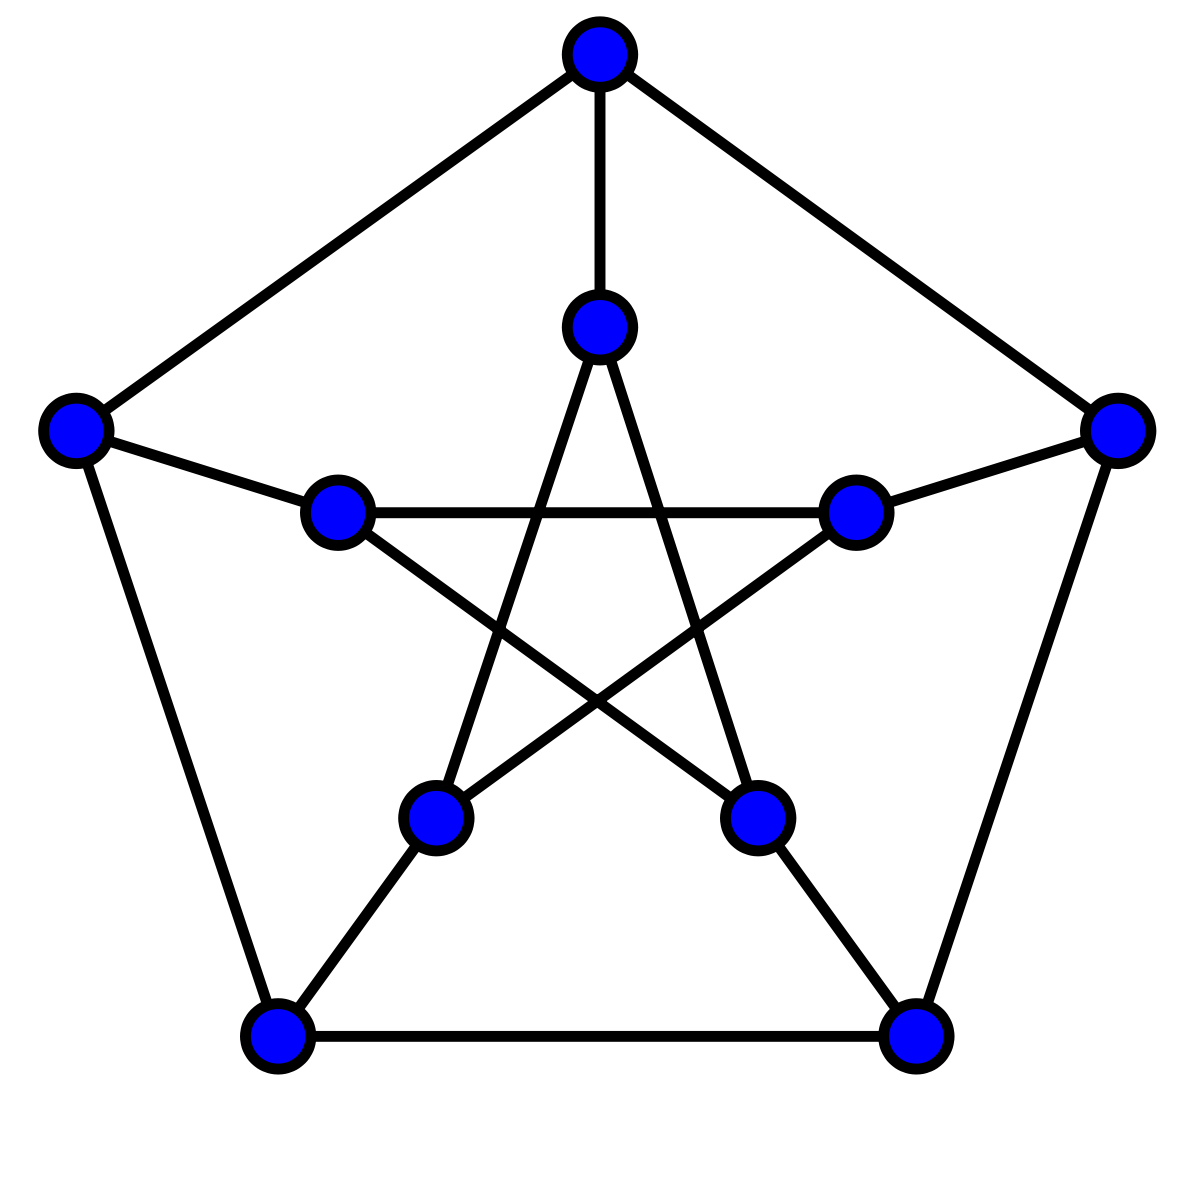
\includegraphics[scale=0.10]{Petersen}
\hspace*{3mm}
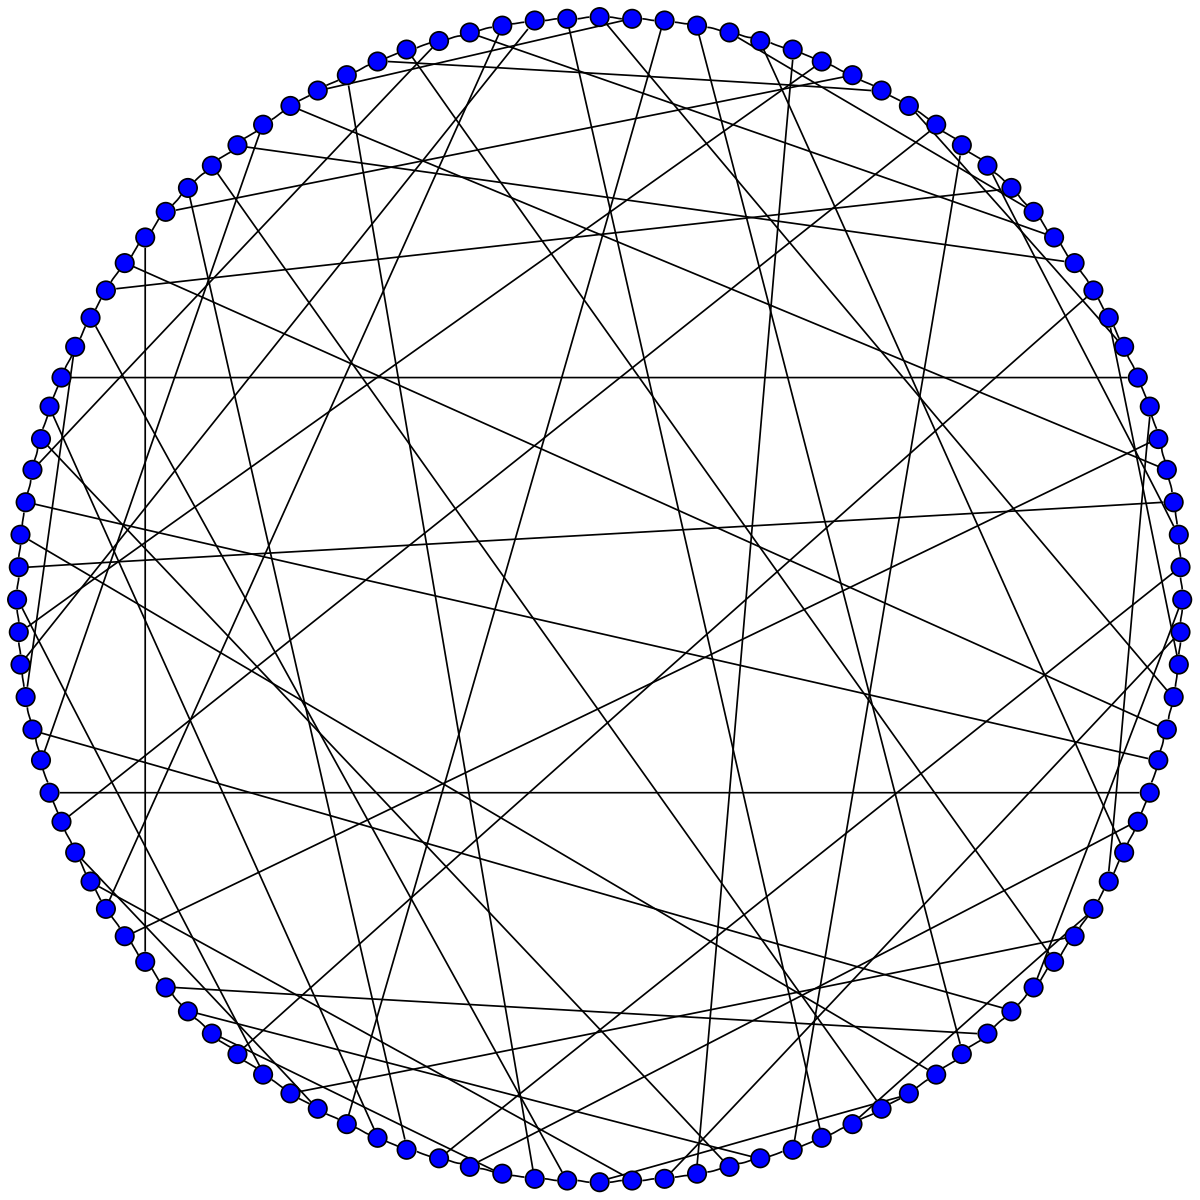
\includegraphics[scale=0.10]{Balaban}
\hspace*{3mm}
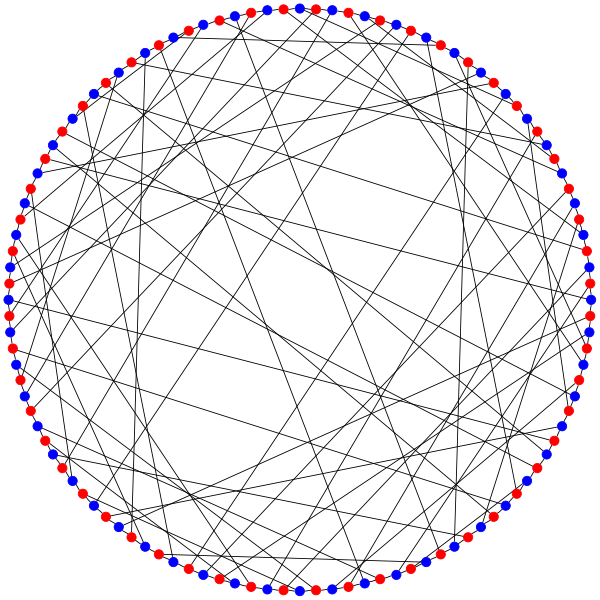
\includegraphics[scale=0.20]{Ljubljana}
\hspace*{3mm}
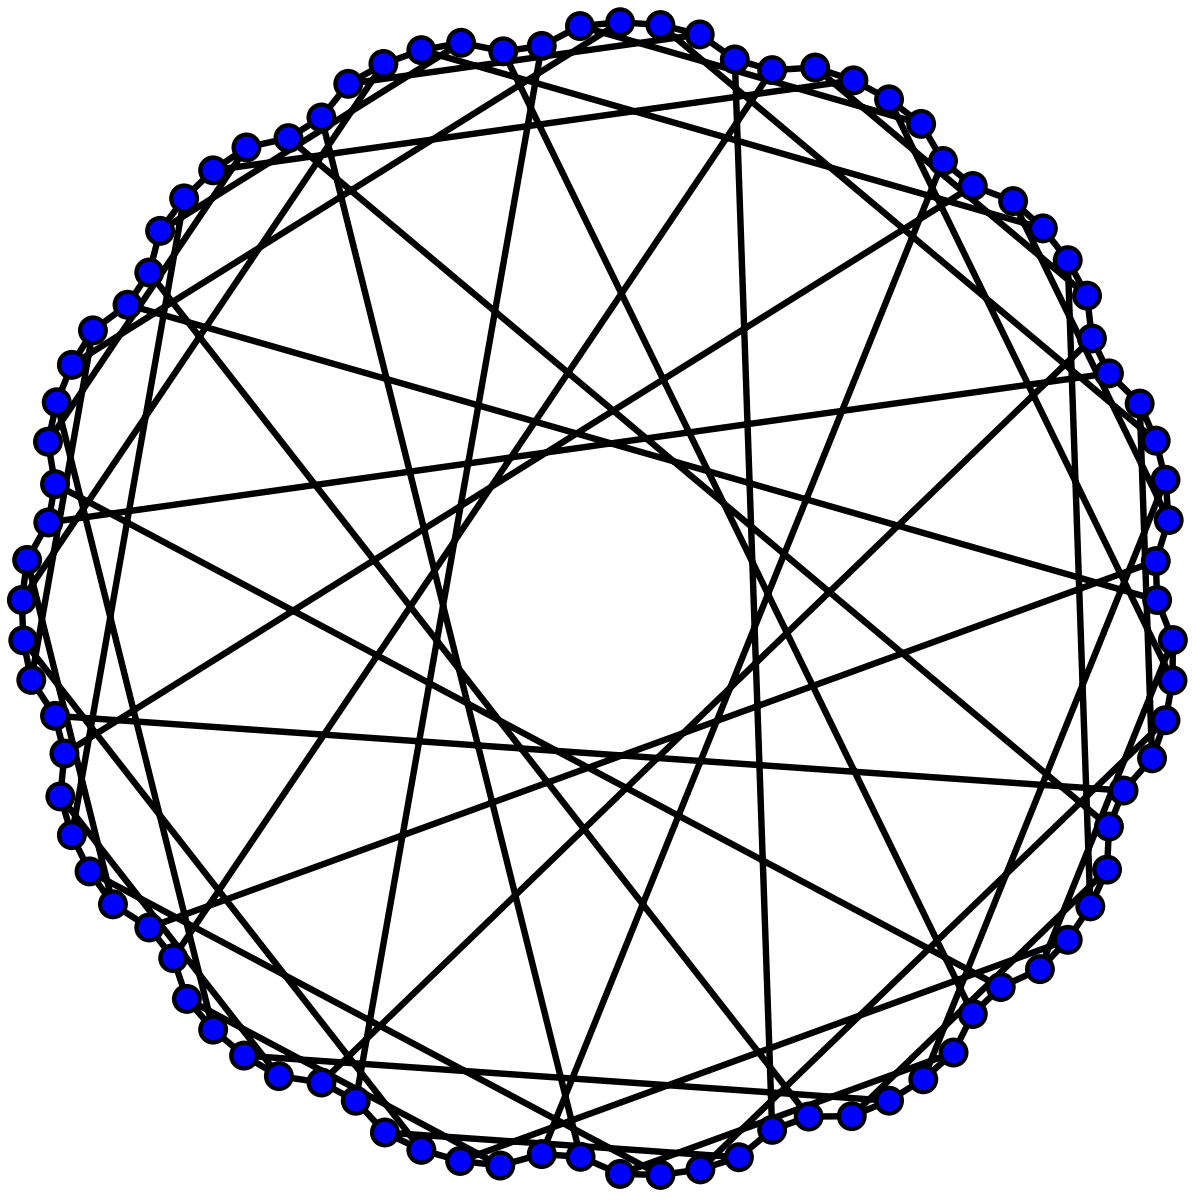
\includegraphics[scale=0.10]{Foster}
\caption{The Petersen, Balaban 11-cage, Ljubljana and Foster graphs. Indeed, the last three graphs will be the hardest for the experiments.}
\end{figure}
\end{center}

\begin{center}
\begin{table}[h!]
\centering
\begin{tabular}{|c|c|c|c|c|}
\hline
\#graphs & avg/med./max \#vert. & avg/med./max \#edges & avg/med./max $\tw$ \\
\hline \hline
125 & 83.05/25/3282 & 166.63/60/6561 & 9.79/7/29 \\
\hline
\end{tabular}
\captionof{table}{Statistics for the named graphs.}
\end{table}
\end{center}

\subsection{Results}

We ran implementations of both algorithms on all mentioned graphs. We will report the average, median and maximum treewidth/vertex cover size/time for all graphs. The time measurements do not include reading the input graphs and writing solutions. In case of the TD-based algorithm, the runtime includes the conversion of the derived TD to a nice TD and the execution of the dynamic programming algorithm based on nice TDs. 

\begin{center}
\begin{table}[h!]
\centering
\begin{tabular}{|c|c|c|c|c|c|}
\hline
package & \#graphs & avg/med./max $\tw$. & avg/med./max $\VC$ & avg/med./max time[s] \\
\hline \hline
stdlib & 142 & 1.85/2/4 & 18.56/11/269 & 0.0008/0.0003/0.0307 \\
\hline
contiki & 1082 & 1.71/2/7 & 18.07/9/728 & 0.0007/0.0002/0.1559 \\
\hline
fuzix & 529 & 1.97/2/6 & 20.76/12/295 & 0.0008/0.0003/0.0339 \\
\hline
\end{tabular}
\captionof{table}{Results for the considered CFGs.}
\end{table}
\end{center}

The computations of the TD-based algorithm on the test set of CFGs take less than a second in total, which is due to the fact that most CFGs have treewidth lower than 2 and are small (compare with Table \ref{stat_CFGs}). The paper about the treewidth of C proves that CFGs without \emph{goto} statements have treewidth at most 7 \cite{Ctree}. We used methodes included in TdLib that are exact for CFGs without \emph{goto} statements. More precisely, exact reduction rules that reduce graphs of treewidth at most $4$ to the empty graph, a generic heuristic and a postprocessing based on triangulization minimization are used. They have running time $\mathcal{O}(n^{3}), \mathcal{O}(n^{3})$ and $\mathcal{O}(n)$ respectively. The authors of the paper included this "pipeline" in compilers for the computation of several NP-hard problems that occur in them, e.g. register allocation.  

\begin{center}
\begin{table}[h!]
\centering
\begin{tabular}{|c|c|c|c|c|}
\hline
$n$ & avg/med./max $\tw$. & avg/med./max $\VC$ & avg/med./max time[s] \\
\hline \hline
50 & 3.66/2/15 & 12.23/12/27 & 0.1347/0.0012/2.6110 \\
\hline
100 & 4.46/3/15 & 20.35/20/44 & 0.2666/0.0019/11.5305 \\
\hline
200 & 5.07/3/15 & 34.99/33/69 & 0.7391/0.0033/23.1289 \\
\hline
250 & 5.31/4/15 & 42.45/39/88 & 0.9472/0.0103/24.0645 \\
\hline
500 & 5.95/5/15 & 78.49/72/157 & 2.2913/0.0298/43.4646 \\
\hline
\end{tabular}
\captionof{table}{Results for the considered partial $k$-trees grouped by $n$.}
\end{table}
\end{center}

By investigating the results for the partial $k$-trees grouped by $n$, we see that the running time of the TD-based algorithm depends linear (and not exponential) on $n$.

\begin{center}
\begin{table}[h!]
\centering
\begin{tabular}{|c|c|c|c|c|}
\hline
package & avg/med./max $\tw$. & avg/med./max $\VC$ & avg/med./max time[s] \\
\hline \hline
1 & 0.97/1/1 & 18.33/11/86 & 0.0042/0.0029/0.0130 \\
\hline
2 & 1.4/1/2 & 26.07/19/117 & 0.0036/0.0022/0.0127 \\
\hline
3 & 1.75/2/3 & 29.4/19/118 & 0.0043/0.0028/0.0195 \\
\hline
4 & 2.3/2/4 & 33.05/23/129 & 0.0064/0.0031/0.0309 \\
\hline
5 & 2.76/2/5 & 34.94/24/134 & 0.0096/0.0038/0.0525 \\
\hline
6 & 3.43/3/6 & 37.14/27/143 & 0.0171/0.0045/0.1015 \\
\hline
7 & 4.09/4/7 & 38.28/29/146 & 0.0308/0.0081/0.1774 \\
\hline
8 & 4.79/5/8 & 39.62/30/144 & 0.0542/0.0116/0.4428 \\
\hline
9 & 5.31/6/9 & 41.00/32/144 & 0.1058/0.0150/0.9290 \\
\hline
10 & 6.06/7/10 & 42.64/32/148 & 0.1780/0.0280/1.3136 \\
\hline
11 & 6.70/8/11 & 42.45/39/88 & 0.3626/0.0272/2.8060 \\
\hline
12 & 7.46/8/12 & 44.33/35/147 & 0.7838/0.03882/8.2476 \\
\hline
13 & 8.04/9/13 & 44.92/35/154 & 1.5113/0.0586/12.1212 \\
\hline
14 & 8.82/10/14 & 45.42/36/146 & 3.7556/0.1338/42.6301 \\
\hline
15 & 9.45/11/15 & 47.46/38/157 & 6.2944/0.2169/44.1330 \\
\hline
\end{tabular}
\captionof{table}{Results for the considered partial $k$-trees.}
\end{table}
\end{center}

The situation is different when the results are grouped by $k$. Recall that on each bag of a TD exponentially (in the size of the bag) many intermediate results are computed and stored. For a graph of treewidth $k-1$, there exists a bag of size $k$ in an optimal TD. At this bag, $2^{k}$ intermediate results are computed. This fact is reflected in the running time of the TD-based algorithm, which is more or less doubling when incrementing $k$.

TODO: named graphs

\section{Summary}

We experimentally showed that TD-based algorithms may be of practical use for solving NP-complete problems, here the vertex cover problem, on graph classes of bounded treewidth by comparing a standard exponential-time algorithm with an TD-based dynamic programming algorithm on control flow graphs derived from various C functions and random partial $k$-trees for small $k$, both having small treewidth. Furthermore we tested both algorithms on famous graphs, i.e. having a name; this test set contains graphs of prohibitively high treewidth, such that some graph have to be excluded for our experiments. Nevertheless, an optimal solution for the vertex cover problem could be computed in reasonable time by the TD-based algorithm for graphs having treewidth up to 29. The exponential time algorithm performs poorly on most graphs, because it does not make use of the special structure of graphs having low treewidth. Neglecting structural properties of graphs arising from treewidth, it exponentially depends on the size of input graphs, hence having no chance to deal graphs with a "large" number of vertices.

\bibliographystyle{unsrt}

\begin{thebibliography}{9}

\bibitem{karp} Karp, R. M. (1972). Reducibility Among Combinatorial Problems.. In R. E. Miller \& J. W. Thatcher (eds.), Complexity of Computer Computations (p./pp. 85-103), : Plenum Press, New York. ISBN: 0-306-30707-3

\bibitem{wiki} The vertex cover problem, \url{https://en.wikipedia.org/wiki/Vertex_cover}

\bibitem{Diestel} Diestel, R. (2005). Graph Theory. Springer-Verlag Heidelberg, New York. 

\bibitem{survey} H. L. Bodlaender (1993), A tourist guide through treewidth, Acta Cybernetica, Vol. 11

\bibitem{graphminor} Neil Robertson and P.D Seymour (1991), Graph minors. I. Excluding a forest, Journal of Combinatorial Theory, Series B, Vol. 35, pp 39 - 61

\bibitem{arnborg} Stefan Arnborg (1985), Efficient Algorithms for Combinatorial Problems with Bounded Decomposability, BIT, Vol. 25, pp 2--23

\bibitem{sage} SageMath, \url{http://www.sagemath.org/}

\bibitem{Patric} Patric R.J. Östergård (2002), A fast algorithm for the maximum clique problem. Discrete Applied Mathematics, Vol. 120, pp 197-207

\bibitem{Ctree} Krause P., Larisch L. (2017), The treewidth of C, submitted

\bibitem{TdLib} Larisch L, TdLib, \url{https://github.com/freetdi/tdlib}

\bibitem{PACE_2017} The PACE 2017 challenge, \url{https://pacechallenge.wordpress.com/pace-2017/track-a-treewidth/}

\bibitem{Fuzix} Fuzix, \url{https://github.com/EtchedPixels/FUZIX}

\bibitem{contiki} Adam Dunkels and Björn Grönvall and Thiemo Voigt (2004): Contiki - a Lightweight and Flexible Operating System for Tiny Networked Sensorss Proceedings of the First IEEE Workshop on Embedded Networked Sensors (Emnets-I)

\bibitem{named_graphs} Named graphs, \url{https://github.com/freetdi/named-graphs}

\bibitem{CFGs} Control flow graphs, \url{https://github.com/freetdi/named-graphs}


\end{thebibliography}

\newpage

\section{Appendix}


\begin{algorithm}[h!]
\caption{max-Clique algorithm}
\begin{algorithmic}[1]

\State{/* global variables */}
\State{$c[i]$ table, found bool, max integer}
\State{}

\Function{start}{}
\State{max := 0}
\For{i:=n to 1}
\State{found := false}
\State{clique($S_{i} \cap N(v_{i})$, 1)}
\State{c[i] := max //largest clique in $S_{i}$}
\EndFor
\EndFunction

\State{}

\Function{clique}{$U$, size}

\If{$U = \emptyset$}
\If{size $>$ max}
\State{max := size}
\State{save new record}
\State{found := true}
\EndIf
\State{\Return}
\EndIf

\While{$U \not = \emptyset$}

\If{size + $|U| \leq $ max}
\State{\Return}
\EndIf

\State{$i := \min\{j: v_{j} \in U\}$}
\If{size + $c[i] \leq $ max}
\State{\Return}
\EndIf

\State{$U := U \backslash \{v_{i}\}$}
\State{clique($U \cap N(v_{i}),$ size +1)}

\If{found == true}
\State{\Return}
\EndIf
\EndWhile

\EndFunction
\end{algorithmic}
\end{algorithm}

\begin{table}[h!]
\centering
\begin{tabular}{|c|c|c|c|}
\hline
name & $|V|$ & $|E|$ & $\tw$ \\
\hline \hline
BrouwerHaemersGraph & 81 & 810 & 54 \\
\hline
CameronGraph & 231 & 3465 & 177 \\
\hline
Cell120 & 600 & 1200 & 112 \\
\hline
DejterGraph & 112 & 336 & 42 \\
\hline
FoldedCubeGraph\_7 & 64 & 224 & 31 \\
\hline
GossetGraph & 56 & 756 & 44 \\
\hline
HallJankoGraph & 100 & 1800 & 87 \\
\hline
HigmanSimsGraph & 100 & 1100 & 77 \\
\hline
HyperStarGraph\_10\_5 & 252 & 630 & 84 \\
\hline
JohnsonGraph\_10\_4 & 210 & 2520 & 140 \\
\hline
KneserGraph\_10\_2 & 45 & 630 & 35 \\
\hline
KneserGraph\_8\_3 & 56 & 280 & 34 \\
\hline
M22Graph & 77 & 616 & 55 \\
\hline
NonisotropicUnitaryPolarGraph\_3\_3 & 63 & 1008 & 55 \\
\hline
OddGraph\_5 & 126 & 315 & 48 \\
\hline
PasechnikGraph\_2 & 49 & 441 & 38 \\
\hline
PasechnikGraph\_3 & 121 & 3025 & 104 \\
\hline
SimsGewirtzGraph & 56 & 280 & 36 \\
\hline
SquaredSkewHadamardMatrixGraph\_2 & 49 & 588 & 41 \\
\hline
SquaredSkewHadamardMatrixGraph\_3 & 121 & 3630 & 109 \\
\hline
SwitchedSquaredSkewHadamardMatrixGraph\_2 & 50 & 525 & 40 \\
\hline
SwitchedSquaredSkewHadamardMatrixGraph\_3 & 122 & 3355 & 109 \\
\hline
SymplecticDualPolarGraph\_4\_4 & 85 & 850 & 64 \\
\hline
SymplecticPolarGraph\_4\_4 & 85 & 850 & 64 \\
\hline
T2starGeneralizedQuadrangleGraph\_4 & 64 & 576 & 47 \\
\hline
\end{tabular}
\captionof{table}{Named graphs of $\tw > 30$ that we did not consider for our experiments.}
\end{table}


\end{document}
\grid
\grid
